% Supplementary details for the final paper: method, results, limitations and process text that the paper does not carry.
\documentclass[manuscript,screen]{acmart}

\usepackage{longtable}
\usepackage{graphicx}
\graphicspath{{figures/}}

\setcopyright{none}
\settopmatter{printacmref=false}
\renewcommand\footnotetextcopyrightpermission[1]{}
\acmConference[CSE 216 / COGS 230]{Final paper}{Fall 2026}{}
\acmYear{2026}
\acmDOI{}
\acmISBN{}

\newcommand{\code}[1]{\texttt{#1}}

\begin{document}
\title[Offloading or Surrendering? Supplementary Details]{Supplementary Details for ``Offloading or Surrendering?''}
\author{Wayne Wang}
\affiliation{\institution{CSE 216 / COGS 230, Fall 2026}\city{[city]}\country{USA}}
\maketitle
\renewcommand{\thefigure}{S\arabic{figure}}\renewcommand{\thetable}{S\arabic{table}}

This file holds the full data funnel, coding procedure, further results, further limitations and process record behind the paper. Like the paper, it contains no dataset text, narratives are paraphrases, and every label comes from AI coders.

\section{Method Details}

\subsection{Data and screening}

The NIRVANA task was about 30 minutes long; 24 essays have logged times beyond that, the longest 5,010 seconds. What the original authors did is reported only as far as their papers state it and as far as the agents read them, as recorded in the read levels in the supplementary materials. Survey, interview and consent appendices do not apply, because none was created.

Samples of WildChat-1M were screened by an LLM for formal long-form writing: an extended formal text such as an essay, research paper, report, thesis, literature review, proposal or business plan, article for publication (including expository blog articles) or formal statement. Fiction, emails, CVs, marketing copy, code and translation-only work were excluded. The definition was committed before any record was labeled. Figure~\ref{fig:flow} shows the resulting sets. Of 837,989 records, 139,736 were eligible: English, at least two non-blank user turns, and deduplicated. A random seed of 1,200 eligible conversations was labeled by an LLM, and 120 (10.0\%) were included, 114 of which passed a rule requiring a user turn after the first writing turn. A logistic-regression ranker over embeddings and keywords was trained on 1,204 labels, and the top 2,500 conversations were confirmed by the LLM, for an accepted pool of 2,236. The coded sample was drawn only from the random seed's 114, one conversation per IP cluster, so the ranking cannot bias it. A separate model audited a random 120 accepted conversations and agreed on 118 (98.3\%). Nine of the 35 coded conversations were screened as articles, and all 3 that the audit rejected are in that group.
% src: wildchat/REPORT.md Funnel, Precision and recall, Sample

\begin{figure}[tbp]
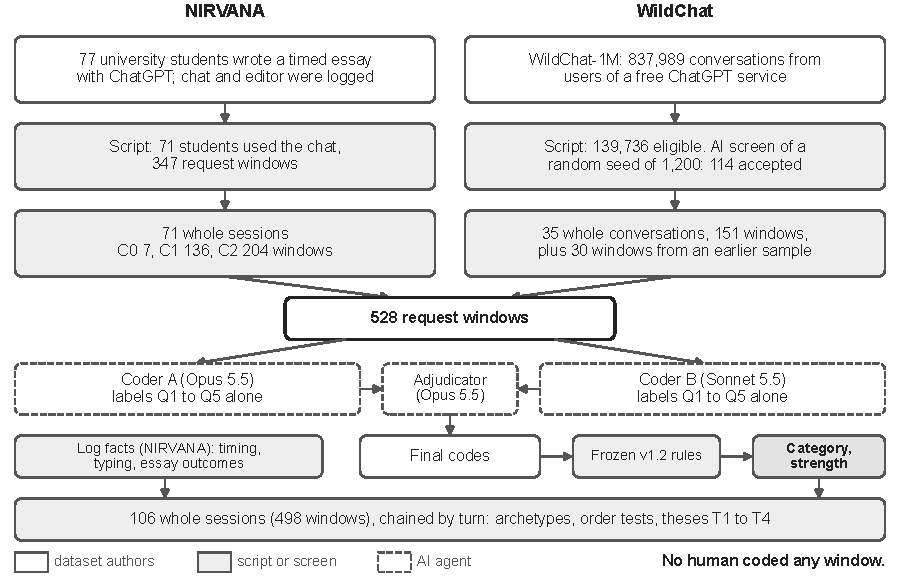
\includegraphics[width=\linewidth]{flow.pdf}
\caption{How the data moved from the two sources to the theses, and who or what did each step. Dashed boxes are AI agents, shaded boxes are scripts or screens, and plain boxes are the dataset authors' work. Coverage \code{C0} is a request and response with no usable next action, \code{C1} adds a later chat turn, and \code{C2} adds editor actions. Three WildChat conversations are capped at ten turns and remain in the session measures; the 30 earlier windows are incomplete and stay out of every session measure.}
\Description{A flow chart. NIRVANA: 77 students, then 71 who used the chat with 347 windows, then 71 whole sessions. WildChat: 837,989 conversations, then 139,736 eligible and 114 accepted from a random seed of 1,200, then 35 whole conversations with 151 windows plus 30 earlier windows. Both feed 528 request windows, coded separately by Coder A (Opus 5.5) and Coder B (Sonnet 5.5), with an adjudicator (Opus 5.5) resolving disagreements. Final codes pass through frozen v1.2 rules to one category and strength. Categories and NIRVANA log facts feed analysis of 106 whole sessions and theses T1 to T4. A note says no human coded any window.}
\label{fig:flow}
\end{figure}
% src: data/REPORT.md Coverage; wildchat/REPORT.md Funnel, Sample; analysis/results/out_of_sample.md s4

Scripts scan the repository for leaked dataset text, and WildChat contact patterns were masked before any reading.

\subsection{Theoretical grounding and codebook development}

The stages of writing come from \citet{flower1981}, read secondhand through work that builds on them \cite{jelson2026chi,reza2025}. \citet{bastani2025} was read as its working-paper version.

Codebook v1.0 was a reconstruction from the proposal and Milestone 1. Agents revised it through four pilot rounds, 132 windows, plus a 10-window check of one rule and 12 constructed cases, on windows that share no session with the 100-window sample and the 20-window set; later whole-session coding did include pilot sessions. Two AI coders applied each round. Version 1.1 cut two labels that the pilots did not support and added \code{U8} and \code{prior\_own\_work}. Version 1.1 was frozen on November 6, 2026, with round 4 agreement of $\kappa = 0.78$ on \code{decision}, 1.0 on \code{verification} and 0.94 on \code{uptake}.
% src: codebook/REPORT.md; CSE216_Research_Writing_Codebook_v1.0.md header

\begin{figure}[tbp]
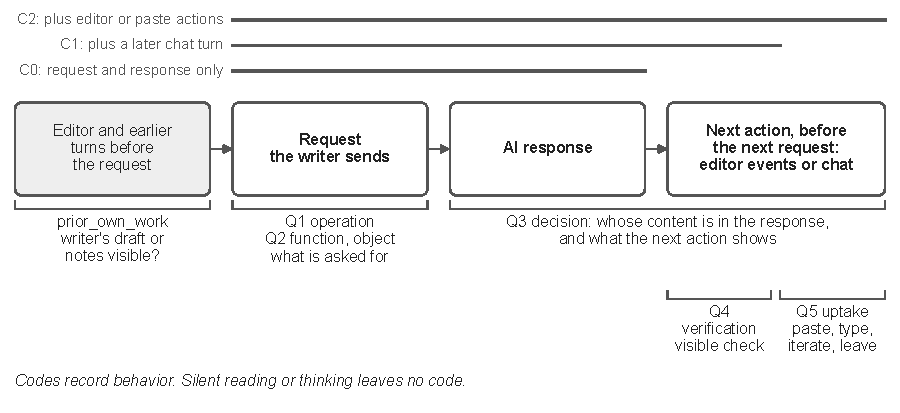
\includegraphics[width=\linewidth]{anatomy.pdf}
\caption{Anatomy of a window, the unit of coding. Each code is read from a named part of the window. The lines above show what each coverage level lets a coder see: a chat-only window (\code{C1}) has no editor actions, so it cannot show pasting or typing.}
\Description{Four boxes in sequence: editor and earlier turns before the request, the request, the AI response, and the next action before the next request. Brackets below show that prior own work is read from the first box, Q1 operation and Q2 function and object from the request, Q3 decision from the response and the next action, and Q4 verification and Q5 uptake from the next action only. Lines above show that C0 covers request and response, C1 adds a later chat turn and C2 adds editor actions.}
\label{fig:anatomy}
\end{figure}
% src: codebook/CSE216_Research_Writing_Codebook_v1.1.md s1, s2

\subsection{Coding procedure}

All windows were coded by AI agents in Claude Code. Coder A was Claude Opus 5.5 and Coder B was Claude Sonnet 5.5. Fresh agents worked on separate batches with sessions kept whole. They were instructed not to read each other's labels, and a transcript audit found that none did; the file system did not enforce this. Where they disagreed, a fresh Opus 5.5 adjudicator ruled between two labels shown with a seeded order flip that hid which coder was which. Temperature cannot be set in this tool, so labels are saved rather than regenerated. Briefs and prompts are in the supplementary materials. Transcripts were audited by script for each agent's file access and served model.

Coding ran in three stages. The first took a sample of 100 windows (70 NIRVANA and 30 WildChat) from 37 sessions, with coders shown the last three earlier turns. The second coded all remaining NIRVANA windows under full history, reading one turn at a time and labeling each before opening the next, and recoded the 18 earlier windows with older unseen turns under a rule fixed in advance. It used 41 agents. The third coded the 35 WildChat conversations in the same way. A Claude Fable 5.1 agent separately coded a 20-window set that had been reserved for human coding. That comparison is a third AI consistency check and not human validation. the Barriers section of the paper explains why it replaced a human.
% src: coding/REPORT.md; sessions/REPORT.md; wildchat/REPORT.md

\subsection{Rule strength and review}

Strength is \emph{strong} when the window shows a signature a source names and coverage can see it, \emph{moderate} when one element is unobservable or a live alternative remains, and \emph{weak} when the match is only by request type or rests on a study of another task. A reviewing agent enumerated all 98,000 code combinations and found no errors.

\subsection{Analysis method and tools}

The qualitative analysis was deductive: categories were fixed by the rule table before the new labels were read, and session types were then derived from the data. Agreement is Cohen's $\kappa$, with bootstrapped intervals over 2,000 draws and sessions as the resampling unit where sessions matter; prior studies that code prompts also report $\kappa$ \cite{jelson2026chi,poquet2026}. Order claims are tested against a within-session shuffle, reordering each session's categories 2,000 times, which holds a session's make-up fixed and moves only its order. Outcome links are Spearman correlations with two-sided permutation $p$ values across sessions. Session archetypes come from optimal-matching distance between category sequences and average-linkage clustering, with the number of clusters chosen by best mean silhouette over 3 to 7. A logistic regression with 1,000 session-cluster bootstraps tests the next-window prediction.
% src: analysis/results/mining.md preamble, s1, s3, s8; sessions/REPORT.md

Agents worked in Claude Code. Analysis scripts are Python, with NumPy and Matplotlib; the WildChat ranker used the \code{BAAI/bge-small-en-v1.5} embedding model. Data preparation, coding and analysis ran on November 6--7, 2026, and this draft was written on November 8. Each stage's numbers rerun from saved labels by script, with no model calls, and repeat runs gave byte-identical outputs; numbers in the schematic figures and some figure labels are typed from those results files. Fresh agents with no access to the working agent's reasoning checked each stage against a stated gate, and a skeptic agent tried to refute each claim in the results.
% src: analysis/scripts/run_all.sh; analysis/SKEPTIC_T.md; git log dates


\section{Further Results}

\subsection{Categories}

\begin{figure}[tbp]
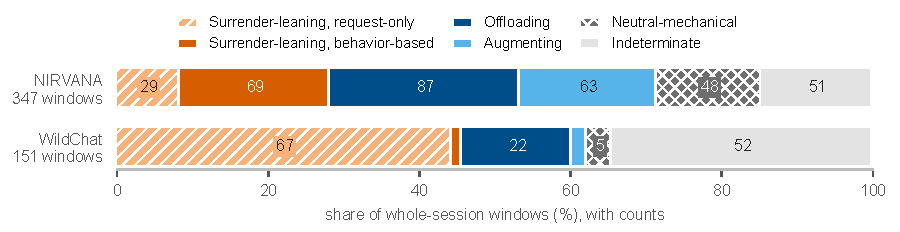
\includegraphics[width=\linewidth]{categories.pdf}
\caption{Category of each whole-session window, by dataset. WildChat's surrender-leaning windows are almost all request-only, because a chat log cannot show what happened to the text. Unlabeled WildChat segments are behavior-based, 2, and augmenting, 3.}
\Description{Two stacked horizontal bars. NIRVANA, 347 windows: request-only 29, behavior-based 69, offloading 87, augmenting 63, neutral-mechanical 48, indeterminate 51. WildChat, 151 windows: request-only 67, behavior-based 2, offloading 22, augmenting 3, neutral-mechanical 5, indeterminate 52.}
\label{fig:categories}
\end{figure}
% src: analysis/results/mining.md s5 tokens; analysis/results/out_of_sample.md s7c


Session e70 shows the turn within one session. The writer first hands over their own paragraphs for polishing, then asks for text they do not have, and pastes it unchanged. Five windows ask the AI to check itself (\code{V2}), and the 13 reasoned challenges fall in 6 sessions.

\subsection{Further results for the theses}

T1: both behavior-based surrender correlations (AI share, ownership) hold on multi-window sessions alone (0.54 and $-0.49$).

\begin{figure}[tbp]
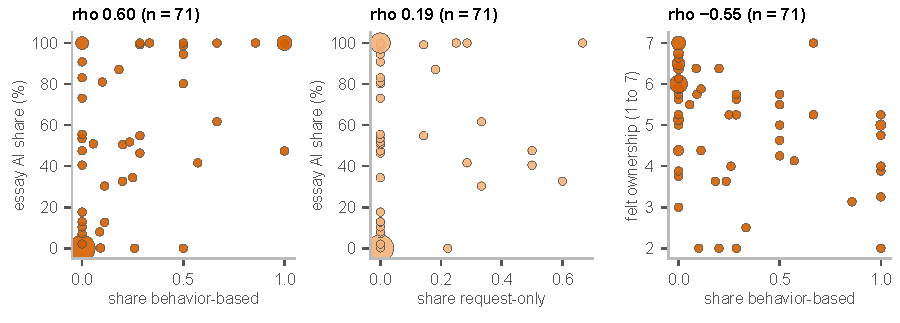
\includegraphics[width=\linewidth]{outcome.pdf}
\caption{NIRVANA essay outcomes by session. Behavior-based surrender tracks the essay's AI share and lower ownership. Request-only surrender tracks the AI share only weakly, and 58 of the 71 sessions have a request-only share of zero. Larger markers stand for several sessions at one point.}
\Description{Three scatter plots across 71 sessions. Left: share of windows surrender-leaning by behavior against GPT Final percent, rho 0.603. Middle: share by request only against GPT Final percent, rho 0.191. Right: share by behavior against Perceived Ownership, rho minus 0.546.}
\label{fig:outcome}
\end{figure}
% src: analysis/results/mining/outcome_sessions.csv; analysis/results/mining.md s8

Substitution sits with requests for generated prose. Pooled across both datasets, 79.5\% of translating-stage (drafting) windows are surrender-leaning, against 22.9\% of planning and 17.4\% of reviewing windows, shares taken over windows with a surrender or support category. In these codes drafting nearly equals generation: 192 of 195 drafting windows are generation requests. The informative result is on the other side. Requests that are not for generated prose are rarely surrender-leaning at any stage (7.1\% when planning, 9.8\% when reviewing). Planning requests come earlier in sessions and reviewing requests later than chance (mean position 0.412 and 0.562; both $p < 0.001$).
% src: analysis/results/mining.md s4, s10

Sessions move across the boundary in recognizable ways. Moves from support into the surrender-leaning category most often land on a generation request iterated in chat (18 of 29). Moves back out most commonly land on the writer revising AI text in the editor (8 of 29, the plurality; 27 of the 29 exits are in NIRVANA).
% src: analysis/results/mining.md s3

T2: the anchor also predicts the next step. In a model of the next substantive window, a visible draft predicts lower odds of a surrender-leaning window (odds ratio 0.23, 95\% session bootstrap 0.07 to 0.44), with the current window's category, chat uptake, dataset and position in the model; the rate is 0.21 with a draft and 0.65 without, pooled across datasets, and 0.237 against 0.505 in NIRVANA alone. Most of this is between sessions: in the 16 sessions across both datasets where the draft flag varies, the next-window rate is 0.18 with a draft and 0.26 without. A current request-only surrender window is a larger predictor (odds ratio 7.9). In NIRVANA, writers leave the surrender-leaning category in 9 of 17 transitions with their draft visible, 14 of 34 with notes and 4 of 21 with nothing visible, and they enter it from support in 16 of 41 transitions with only notes and 10 of 59 with a draft. Sessions that become surrender-leaning return to support in 17 of the 29 NIRVANA sessions with a later window and 2 of 21 in WildChat. The document itself grows through a session: NIRVANA's median editor length at the time of a request rises from 101 characters in the first fifth of a session to 2,157 in the last.
% src: analysis/results/mining.md s3, s5, s6

T3: the dwell gap (behavior-based alone 65.4 seconds, $p = 0.0035$) appears in every fifth of a session and within 13 of the 17 sessions that have both kinds. Twenty of 69 behavior-based surrender windows and 31 of 87 offloading windows are copied within 10 seconds. Felt ownership is lower in sessions with more of either kind of surrender ($\rho = -0.55$ behavior-based, $p < 0.001$; $-0.33$ request-only, $p = 0.004$), mostly as a difference between sessions with any behavior-based surrender and those with none: among the 34 sessions that have some, the correlation is $-0.21$ ($p = 0.25$). A fourth log-only rule, a paste followed by a quick return, is precise (66.7\%) but catches only 14.3\%.

\subsection{RQ2 patterns}

\begin{table}[tbp]
\caption{Likely visibility of substitution patterns to the writer (analytic).}
\label{tab:rq2}
\small
\begin{tabular}{p{0.33\linewidth}p{0.17\linewidth}p{0.39\linewidth}}
\toprule
Pattern & Likely noticed? & Why \\
\midrule
Whole paste of AI text (\code{D4 V0 U1}, 32 windows) & Origin yes; missing reasoning no & Pasting is deliberate and ownership is lower, but the writer types almost nothing afterward \\
Surface-only iteration on an AI draft (\code{D2 V1 U4}, 30 windows, 21 surrender-leaning) & Less likely & The writer is busy with length and tone, which feels like editing \\
Ideas from a generation request, written up in the writer's words (\code{D2 U7}, 52 windows, 37 augmenting by the rules; possible substitution of the ideas, which the rules cannot see) & Least likely & The writer types, so ownership need not fall, as with planning or reviewing use \cite{jelson2026chi}, and influence can go unnoticed \cite{bhat2026}. The codebook cannot see the origin of ideas, by design \\
Request-only delegation in chat (R16) & Unknown & The log ends at the request, and the text may be used off-screen \\
\bottomrule
\end{tabular}
\end{table}
% src: analysis/results/patterns.md s1; analysis/THESES.md RQ2 argument

\subsection{The framework against the success criterion}

The proposal's success criterion asked for a framework that assigns real interactions to these categories with acceptable agreement and distinguishes cases that existing frameworks cannot. The first part is met within the limits in the Limitations section of the paper: 78.5\% of new windows receive a category by frozen rules, and AI-to-AI category agreement across all 528 windows is $\kappa = 0.86$. The second part is not established. An agent's comparison across 11 case pairs, written before any real window was coded, rated the project the only framework able to separate 3 of them. NIRVANA's own metrics already separate 2 of those, and the third was built from the codebook's own worked examples, so the project could not have failed it. What the framework adds is narrower. On real data, the distinction that does the most work is one that theory already states: whether a claim was the writer's and reworded, or the AI's and adopted. The addition is making it observable on the same act of pasting, through the code for whose content it is and the typing that follows. Both ends of that contrast occur on real windows: the rules send 30 of 32 whole pastes to the surrender-leaning side and 44 of 52 ask-then-write-own windows to the support side. NIRVANA's essay metric also separates those two, and what the log adds is the typing that follows a paste.
% src: lit/framework_comparison.md; report/M2_draft.md s4; analysis/results/patterns.md s1

The findings suggest specific changes for a future version: split R16, since request-only surrender tracks outcomes weakly and half of the 96 such windows are requests whose output was not used; add a field for work after the response; narrow the rule for unsettled fields; and add a length rule for \code{U3} against \code{U7}. These are proposed and were not applied.

\section{Further Limitations}

\paragraph{Adjudicators lean toward one model.} Where the coders disagreed, the Opus adjudicator sided with Opus Coder A by 25 to 13, 159 to 45 and 54 to 17 across three runs. On the 57 windows where A's and B's categories differ, the final category follows A in 44 and B in 12. Contested labels are therefore A-leaning, although totals barely move: 177 surrender-leaning windows in whole sessions under A's labels, 167 under B's and 167 in the final set.
% src: coding/REPORT.md; sessions/REPORT.md; wildchat/REPORT.md; analysis/results/out_of_sample.md s7

\paragraph{Tests are uncorrected.} The analysis ran 40 category n-gram tests, 29 signature n-gram tests, 20 latency contrasts, 12 outcome correlations and 4 log-only rules without correction for multiple comparisons. The theses rest on the large effects, not on $p$ values near 0.05. The overrepresentation of request-only runs ($p = 0.025$) is one of 40 tests and is about what chance would give.

\paragraph{Sample and generalization.} NIRVANA is one timed essay by university students. WildChat conversations are English, from anonymous users of a free ChatGPT service, drawn from the conversations an LLM accepted in a random seed of 1,200; recall of the larger accepted pool, which was not coded, is about 12\%. An audit questioned 3 of the 35 coded conversations. Windows cluster within sessions: the 21 long working sessions hold 218 of the 498 windows. Archetype structure is modest (best silhouette 0.25), although stable at 89 to 98\% of session pairs when the number of clusters changes. Nothing here speaks to habits over weeks, to skill change, or to research writing specifically, and the demographics of these writers are not analyzed.

\paragraph{Procedure.} Some procedural details reduce what the rule freeze can prove. Final labels for later windows were in git when the rule table was last frozen, and the record that no agent read them rests on agents' briefs and on mapping each late change to a critic finding. Fifty-two NIRVANA windows keep labels coded from shorter views, and a small share of labels rest on reading outside the protocol. Agreement on \code{verification} for editor windows is weak (0.48, interval 0.17 to 0.69), and 20 windows with an unsettled field go to indeterminate as the frozen rules require. \code{V2} to \code{V4} occur so rarely that the framework's distinction between kinds of check has little data behind it. The comparison with existing frameworks reflects ratings by the project's own agent, corrected by a critic.
% src: inference/FROZEN.md; sessions/REPORT.md; wildchat/REPORT.md; analysis/results/out_of_sample.md s5

\section{Process Record}

\paragraph{The promise to be the primary coder was reversed.} My proposal said ``I remain the primary coder,'' with an LLM as a consistency check. On November 6 I chose agent-led work and kept a blind human coding set of 20 windows. The instructions for that set estimated 90 minutes to 2 hours, not the planned hour, and said the task could not be delegated. I delegated it anyway, to a Fable 5.1 agent. With more time, I would code those 20 windows myself before seeing any AI output. \emph{What I learned:} the one step that later steps could not replace was the one I gave up, and the cost of a human check should be estimated before it is promised.

\paragraph{The research-writing sample fell short and could not be reproduced.} The proposal targeted research writing, and Milestone 1 reported 42 clear and 40 possible candidates from a draw of 2,000 records, pending human verification. A rebuild could not reproduce the counts: the original draw method was lost, a new LLM pass gave 41 clear and 69 possible on the rebuilt draw, and keyword rules gave 3 and 15. Of the 41 clear conversations, 21 were not in English. Milestone 1's count was below the proposal's target of 100 and no person had verified it, and too few genuine research-writing conversations was the risk the proposal had named. On November 7 I widened the scope to formal long-form writing, and an agent wrote and committed the new definition before any record was labeled. \emph{What I learned:} a construct has to be defined and tested for precision before its count is reported.

\paragraph{A priming mistake before blind coding.} A report written for me held the frequency of check codes back until after blind coding, because a critic agent noticed that telling a coder those rates could prime them toward ``no check.'' I nevertheless heard the pilot's frequencies before those 20 windows were coded. This became moot only because I did not then code. \emph{What I learned:} a blind protocol has to cover what is said in conversation with agents, as well as which files can be opened.

\paragraph{A shared git index swept files into one commit.} Parallel agent sessions shared a checkout. On November 7, a checkpoint commit for the rule table swept in 27 WildChat files that another session had staged. Their names were printed, their contents were not opened by that session, and a parent session confirmed that they held no dataset text. Because the rules were meant to be frozen before new labels were read, this needed a logged account rather than a quiet fix. \emph{What I learned:} running work in parallel moves the risk to whatever the workers still share, so commits afterward named their paths.

\paragraph{Sources and search tools refused automated access.} The PubMed Central copy of the Bastani paper was blocked by reCAPTCHA, so agents did not bypass it; they read a working-paper version instead. Google Scholar's \code{robots.txt} disallows automated queries, Semantic Scholar returned HTTP 429 on every query, and SSRN showed a bot check. The logged search used OpenAlex and arXiv, and 11 Scholar queries were listed for a person to run. \emph{What I learned:} the version actually read must be recorded with the citation, because it is not always the version of record.

\paragraph{Early work was lost, and a coder view was too short.} The original proposal-stage files, screening data and pilot cases were lost, so the search protocol was built after the seed list existed, and Milestone 1's ``77 students'' turned out to be 71 students with windows. Separately, coders in the first sample saw only the last three earlier turns, and a gate review showed that 10 windows reused text from AI turns nobody had shown them. The 18 windows with unseen turns were recoded with full history. \emph{What I learned:} keep records of how a selection was made from the first day, and state every limit of what a coder can see, including limits that seem harmless.

\paragraph{Review agents caught real errors.} Gates failed repeatedly: the codebook needed three critic passes, and in the first analysis pass a skeptic refuted 3 of 13 findings, including a persistence effect produced by how the shuffle moved closing-turn windows. A later skeptic reworded 10 of 23 claims. \emph{What I learned:} a fresh reviewer who cannot see the worker's reasoning finds things the worker cannot, and that kind of review should be planned for from the start.

\paragraph{Some agents broke the reading protocol.} One WildChat coder batch read ahead on 24 windows, and its labels were not redone. Two NIRVANA adjudicators each read one later part early, and those rulings were redone by fresh agents with the same result. One WildChat adjudicator read some long parts only partly, and those rulings were not redone. Transcript audits and critic reads of the transcripts found these, except one NIRVANA breach, which its adjudicator reported and the first audit script missed. \emph{What I learned:} a rule enforced only by instruction will sometimes be broken, so the audit has to be planned along with the rule.


\bibliographystyle{ACM-Reference-Format}
\bibliography{refs}
\end{document}
